The people that use a system can be represented by personas. This is done in order to ensure the PACT elements are centered in the design process\kanote{Hvad menes der her?}. Personas are general profiles of different types of users. A persona is a concrete representation of a fictitious person. Personas help the designer by having a specific end user in mind, preventing them designing the system for themselves. Personas are developed through the understanding process and through undertaking a PACT analysis. A part of the persona is a short story of the person trying to achieve a goal using the system in a specific context~\cite{benyon2013designing}.

As part of this project, a persona was made, based on the interviews which were conducted.%\cref{interviewbruger}.
This is Camilla, an average user of the system.

\subsubsection{Camilla}
\begin{figure} [h]
  \centering
  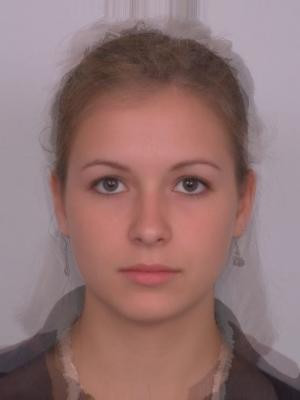
\includegraphics[]{Images/average.jpg}
  \caption{Picture associated with the persona \enquote{Camilla}. Copyright the Face Research Lab. Used with permission.}
  \label{fig:camilla}
\end{figure}
\noindent\textbf{Basic information}
\begin{itemize}
\item 25 years old
\item Medical student
\item Employed in an elderly care center
\item In a relationship with Keith
\item She loves meeting new people
\item When going out she likes to visit small places that allow socialisation
\item Volunteered in Red Cross Uganda
\end{itemize}

It is Friday afternoon and Camilla is planning to meet some of her fellow students at a bar. Camilla and her friends get together after they are finished at school and go to a café to grab a sandwich. After dinner, Camilla takes out her smartphone and checks openPlaylist. Camilla can see that some of her favourite tracks are being played at White Hart, and they agree to go there. Upon arriving Camilla checks in via the application. She immediately notices on the screen behind the bar that the queue is filled with tracks she dislikes. She now uses the application to request and upvote other tracks that she would like to be played. Some other people at White Hart agree on Camilla's choices and they too upvote these tracks. On the screen in the bar Camilla can see some of the other people that upvotes her tracks and later in the evening she meets them and they talk about all the nice music they have in common. Camilla and her new and old friends party all night long and drink a lot of beer.
